% Meridian protocol v13 (shortened run, 34 steps): the finalized tasks and the research behind each one.
% Overleaf: New Project > Upload Project > this file (or paste into main.tex). Compiler: pdfLaTeX.
% No other files are needed; the timeline is drawn with TikZ and the bibliography is built in.
% Every reference was checked against Crossref (or the publisher page) on 2026-09-18; DOIs are listed.
% Items still to fill in are marked \TODO{...} and print in red.
\documentclass[11pt,a4paper]{article}

\usepackage[T1]{fontenc}
\usepackage{lmodern}
\usepackage[margin=2.2cm]{geometry}
\usepackage{microtype}
\usepackage{booktabs}
\usepackage{array}
\usepackage{tabularx}
\usepackage{longtable}
\usepackage{enumitem}
\usepackage{xcolor}
\usepackage{tikz}
\usetikzlibrary{positioning}
\usepackage[most]{tcolorbox}
\usepackage{fancyhdr}
\setlength{\headheight}{14pt}
\usepackage[hidelinks]{hyperref}

\definecolor{ink}{HTML}{1F2A36}
\definecolor{clay}{HTML}{A8543A}
\definecolor{moss}{HTML}{3D6B45}
\definecolor{sky}{HTML}{2F5F8A}
\definecolor{sand}{HTML}{F3EDE3}
\definecolor{amber}{HTML}{C08A1E}

\hypersetup{colorlinks=true,linkcolor=sky,urlcolor=sky,citecolor=moss}
\setlist{itemsep=2pt,topsep=4pt}
\setlength{\parindent}{0pt}
\setlength{\parskip}{5pt}
\renewcommand{\arraystretch}{1.25}

\pagestyle{fancy}
\fancyhf{}
\lhead{\small\color{ink}Meridian protocol: tasks and rationale}
\rhead{\small\color{ink}\nouppercase{\leftmark}}
\cfoot{\small\thepage}

\newcommand{\code}[1]{\texttt{\detokenize{#1}}}
\newcommand{\TODO}[1]{\textcolor{red}{\textbf{[TODO: #1]}}}
\newcommand{\doi}[1]{\href{https://doi.org/#1}{\nolinkurl{doi:#1}}}

\newtcolorbox{notebox}[1]{enhanced,breakable,colback=clay!6,colframe=clay,boxrule=0.5pt,arc=2pt,left=6pt,right=6pt,
  title={#1},fonttitle=\bfseries,colbacktitle=clay,coltitle=white}

% Task description: #1 what the participant does, #2 parameters, #3 what it measures, #4 why (with citations)
\newcommand{\taskdetail}[4]{%
  \begin{tabularx}{\linewidth}{@{}>{\bfseries}p{3.1cm}X@{}}
    Participant does & #1 \\
    Parameters & #2 \\
    Measures & #3 \\
    Why it is here & #4 \\
  \end{tabularx}}

\title{\color{ink}\textbf{Meridian Multimodal Research Platform}\\[6pt]
  \Large The finalized 34-step protocol: tasks, parameters, and their basis in the literature}
\author{Kushagra \\ IIT Ropar}
\date{Protocol version 13 (shortened run) \quad\textbar\quad \today}

\begin{document}
\maketitle
\thispagestyle{empty}

\begin{abstract}
Meridian records a multimodal dataset of emotional and physiological responses: contact sensors (ECG, finger
oximeter, skin conductance), contactless sensors (two face cameras, thermal camera, Wi-Fi channel state
information), and audio, all on one host clock. This document describes the \textbf{finalized shortened protocol
(version 13, ``Shortened run'')}: \textbf{34 steps in about 42 minutes}. Participants watch
six emotion film clips and rate each one; perform two of three between-clip tasks (Stroop, N-back, conversation);
take a word recognition test; read a fixed passage aloud; follow a short controlled-breathing block that provides reference breathing rates
for contactless sensing; and finish with a guided relaxation. For each task it gives the exact parameters
implemented in the software and the published work the design choice rests on.
\end{abstract}

\tableofcontents
\newpage

% ---------------------------------------------------------------------------------------------------------------
\section{The protocol at a glance}

\begin{center}
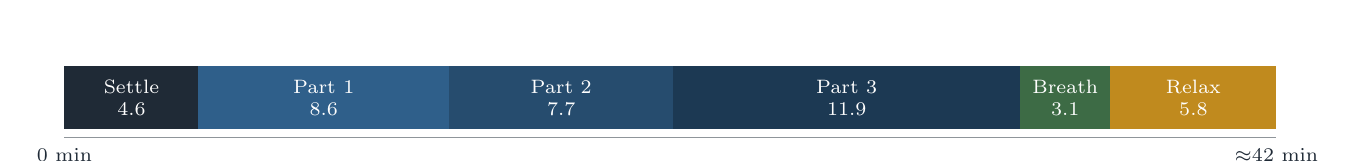
\begin{tikzpicture}[x=0.37cm,y=1cm,every node/.style={font=\scriptsize}]
  % Widths proportional to the estimated minutes of each phase for participant 1 (total 41.6 min).
  \def\ph#1#2#3#4{\fill[#3] (#1,0) rectangle (#2,0.8); \node[white,align=center] at ({(#1+#2)/2},0.4) {#4};}
  \ph{0}{4.6}{ink}{Settle\\4.6}
  \ph{4.6}{13.2}{sky}{Part 1\\8.6}
  \ph{13.2}{20.9}{sky!80!black}{Part 2\\7.7}
  \ph{20.9}{32.8}{sky!60!black}{Part 3\\11.9}
  \ph{32.8}{35.9}{moss}{Breath\\3.1}
  \ph{35.9}{41.6}{amber}{Relax\\5.8}
  \draw[ink!50] (0,-0.1) -- (41.6,-0.1);
  \node[ink,anchor=north] at (0,-0.12) {0 min};
  \node[ink,anchor=north] at (41.6,-0.12) {$\approx$42 min};
\end{tikzpicture}
\end{center}

Table~\ref{tab:plan} is the plan for participant 1, rendered by the software from the saved protocol version 13
(\code{lib/protocol-template.ts}, \code{renderPlan}). The order of the six clips and of the between-clip tasks
changes per participant (Section~\ref{sec:design}); everything else is fixed.

{\small
\begin{longtable}{@{}r p{2.6cm} p{5.0cm} r p{5.3cm}@{}}
\caption{The 34 finalized steps (participant 1). Time is the software's planning estimate in seconds.}\label{tab:plan}\\
\toprule
\# & Phase & Step & Time & Role (key reference) \\
\midrule\endfirsthead
\toprule
\# & Phase & Step & Time & Role (key reference) \\
\midrule\endhead
1 & Getting settled & Sensor and synchronization check & 30 & Verify every stream \\
2 & Getting settled & Current mood (PANAS, start) & 75 & Pre-session mood \cite{watson1988} \\
3 & Getting settled & Personality (TIPI) & 50 & Personality covariate \cite{gosling2003} \\
4 & Getting settled & Resting baseline, eyes open & 120 & Physiological reference \cite{jennings1992,taskforce1996} \\
5 & Part 1 & Emotion clip: happy & 98 & Emotion induction \cite{gross1995} \\
6 & Part 1 & Self-report: happy & 40 & Labels \cite{bradley1994} \\
7 & Part 1 & Neutral washout & 20 & Limit carry-over \cite{rottenberg2007} \\
8 & Part 1 & Emotion clip: sad & 153 & Emotion induction \\
9 & Part 1 & Self-report: sad & 40 & Labels \\
10 & Part 1 & Stroop colour-word task & 90 & Cognitive stress \cite{stroop1935,renaud1997} \\
11 & Part 1 & Workload rating (NASA-TLX) & 45 & Perceived workload \cite{hart1988} \\
12 & Part 1 & Return-to-baseline gate & 30 & Limit carry-over \cite{jennings1992} \\
13 & Part 2 & Emotion clip: disgust & 188 & Emotion induction \\
14 & Part 2 & Self-report: disgust & 40 & Labels \\
15 & Part 2 & Neutral washout & 20 & Limit carry-over \\
16 & Part 2 & Emotion clip: anger & 143 & Emotion induction \\
17 & Part 2 & Self-report: anger & 40 & Labels \\
18 & Part 2 & Return-to-baseline gate & 30 & Limit carry-over \\
19 & Part 3 & Emotion clip: surprise & 188 & Emotion induction \\
20 & Part 3 & Self-report: surprise & 40 & Labels \\
21 & Part 3 & Neutral washout & 20 & Limit carry-over \\
22 & Part 3 & Emotion clip: fear & 100 & Emotion induction \\
23 & Part 3 & Self-report: fear & 40 & Labels \\
24 & Part 3 & Conversation & 180 & Natural speech and motion \cite{busso2008} \\
25 & Part 3 & Word list: study and recognise & 65 & Recognition memory \cite{snodgrass1988} \\
26 & Part 3 & Read aloud & 75 & Read speech, fixed passage \cite{brysbaert2019} \\
27 & Breathing & Seated rest & 20 & Seated anchor \\
28 & Breathing & Box breathing & 64 & Guided slow breathing \cite{balban2023} \\
29 & Breathing & Paced breathing: 6 per minute & 60 & Respiration ground truth \cite{lehrer2014} \\
30 & Breathing & Paced breathing: 20 per minute & 40 & Respiration ground truth \\
31 & Relaxation & Guided body scan & 240 & Low-arousal state \cite{kabatzinn1990} \\
32 & Relaxation & Return to normal & 20 & Final resting reference \\
33 & Relaxation & Current mood (PANAS, end) & 75 & Post-session mood \cite{watson1988} \\
34 & All done & Session complete & 15 & Confirm recordings saved \\
\bottomrule
\end{longtable}
}

\subsection*{Which between-clip tasks each participant does}
The shortened protocol keeps a task slot at the end of Part~1 and Part~3 only; the Part~2 slot was removed. Counterbalancing
still rotates Stroop, N-back, and conversation through the three slots, so the task that lands in the empty
Part~2 slot is not performed. Each task is performed by 24 of every 36 participants. NASA-TLX follows Stroop and
N-back but not the conversation, so the plan has \textbf{34 steps when the conversation is one of the two tasks}
and \textbf{35 steps when the participant does Stroop and N-back} (participants 7--12 and 19--24 in each block of 36).

\begin{center}\small
\begin{tabular}{@{}llll@{}}
\toprule
Participants & Part 1 task & Part 3 task & Not performed \\
\midrule
1--6, 31--36 & Stroop / conversation & conversation / Stroop & N-back \\
7--12, 19--24 & Stroop / N-back & N-back / Stroop & conversation \\
13--18, 25--30 & N-back / conversation & conversation / N-back & Stroop \\
\bottomrule
\end{tabular}
\end{center}

% ---------------------------------------------------------------------------------------------------------------
\section{Design choices that span the whole session}\label{sec:design}

\subsection*{Counterbalancing}
Emotion clip order follows a $6\times6$ Williams Latin square \cite{williams1949}: each emotion appears once in every
position and follows every other emotion exactly once, so first-order carry-over effects are balanced. The order of
the between-clip tasks cycles through six permutations independently, once every six participants, so every
emotion order is paired with every task order across 36 participants. The word list a participant studies is
assigned by a second Latin square over the same $6\times6$ grid, so list difficulty cannot masquerade as an order
effect.

\subsection*{Reproducibility}
Stroop, N-back, and word-test trial lists are generated from a logged random seed, so every participant's exact
trial sequence can be regenerated during analysis. Each session stores a copy of the protocol version and the clip
files it was assigned, so later edits in the protocol builder never alter a recorded session.

\subsection*{Washout and return-to-baseline gates}
Physiological responses to an emotional film outlast the film itself. The protocol therefore separates the two
clips of a block with a 20~s neutral fixation (washout), and ends Parts~1 and~2 with a \emph{return-to-baseline
gate}. The gate needs heart rate within 5~bpm, and skin conductance within 10\%, of the eyes-open resting baseline,
held for 15 consecutive seconds, before the operator advances. Using a measured resting period as the reference,
rather than a fixed pause, follows the cardiovascular baseline literature \cite{jennings1992}, and film-elicitation
guidance recommends neutral periods between clips to limit carry-over \cite{rottenberg2007}.

% ---------------------------------------------------------------------------------------------------------------
\section{The finalized tasks}

\subsection{Sensor and synchronization check (step 1)}
\taskdetail
{Sits still facing the screen.}
{Operator-advanced, about 30~s.}
{Presence and plausibility of every required stream; trigger synchronization.}
{A preflight check before any data that matters is recorded. Not a research task in itself.}

\subsection{Mood and personality questionnaires (steps 2, 3, 33)}
\taskdetail
{Answers PANAS (20 mood adjectives, 5-point scale) at the start and end, and TIPI (10 items, 7-point scale) at the
start.}
{PANAS at steps 2 and 33; TIPI at step 3. Placed \emph{before} the resting baseline so answering does not disturb
it.}
{Positive and negative affect before and after the session; Big-Five personality traits.}
{PANAS is the standard brief measure of positive and negative affect \cite{watson1988}; the pre/post pair checks
whether the session as a whole shifted mood. TIPI measures the Big Five in ten items \cite{gosling2003}, enough to
use personality as a covariate for individual differences in emotional reactivity without a long inventory. Only
instruments usable without licence fees are included.}

\subsection{Resting baseline, eyes open (step 4)}
\taskdetail
{Looks at a fixation cross and breathes naturally for 120~s.}
{Timer-advanced. A resting blood-pressure reading is taken after settling.}
{Resting heart rate, heart-rate variability, skin conductance level, breathing, and face and thermal appearance.}
{Every later response is expressed relative to the participant's own resting state. Heart-rate-variability
standards and psychophysiology recommendations call for a controlled resting recording before any manipulation
\cite{taskforce1996,laborde2017}; a quiet, low-demand resting baseline is also the reference the gates return to
\cite{jennings1992}.}

\subsection{Emotion film clips (steps 5, 8, 13, 16, 19, 22)}
\taskdetail
{Watches six short film clips full screen with sound, one per basic emotion: happiness, sadness, anger, fear,
surprise, disgust.}
{Durations: happy 93~s, sad 148~s, anger 138~s, fear 95~s, surprise 183~s, disgust 183~s (anger and disgust are
the replacement clips). All are H.264 1280$\times$720, 30~fps, AAC 48~kHz. Onset is logged when the video actually
starts playing. Clips are drawn from \TODO{name of the validated film set, with citation}.}
{Emotional responses in every physiological and behavioural channel, time-locked to the clip.}
{Film clips are the most widely used and best validated way to elicit discrete emotions in the laboratory: they
are standardized, dynamic, and ethically acceptable \cite{gross1995,rottenberg2007}. Validated databases supply
normative ratings for each clip \cite{schaefer2010}. The six categories follow Ekman's basic emotions
\cite{ekman1992}. The same paradigm underlies the main affective-computing datasets, DEAP \cite{koelstra2012} and
MAHNOB-HCI \cite{soleymani2012}, which makes Meridian directly comparable to them.}

\subsection{Self-report after each clip (steps 6, 9, 14, 17, 20, 23)}
\taskdetail
{Rates valence, arousal, and dominance; chooses the main emotion felt (six basic emotions or neutral) and its
intensity; says whether the clip was familiar.}
{Self-Assessment Manikin on 9-point scales; intensity on 9 points; familiarity Yes/No/Not sure. About 40~s.}
{Per-clip ground-truth labels, both dimensional and categorical.}
{The Self-Assessment Manikin is a non-verbal, fast, and validated measure of valence, arousal, and dominance
\cite{bradley1994}. Collecting both dimensional and categorical labels, as DEAP and MAHNOB-HCI do
\cite{koelstra2012,soleymani2012}, lets the dataset support both kinds of models and checks whether each clip
elicited its target emotion. Familiarity lets analysis exclude clips the participant had seen before.}

\subsection{Neutral washout (steps 7, 15, 21)}
\taskdetail
{Looks at a fixation cross and breathes normally.}
{20~s, timer-advanced.}
{Decay of the response to the preceding clip.}
{Separates the two clips of a block to reduce carry-over between emotions \cite{rottenberg2007}.}

\subsection{Return-to-baseline gates (steps 12, 18)}
\taskdetail
{Sits quietly and breathes normally.}
{At least 25~s; advances once heart rate and skin conductance are back near baseline (Section~\ref{sec:design}).}
{Whether physiology has recovered before the next block.}
{Prevents the response to one block from contaminating the next \cite{jennings1992,rottenberg2007}.}

\subsection{Stroop colour-word task (between-clip task)}
\taskdetail
{Chooses the \emph{ink colour} of a colour word, ignoring what the word says.}
{30 trials, 15 congruent and 15 incongruent; no more than 3 trials in a row of the same kind; no immediate word
repeats; six colours; 2~s response deadline; 400~ms fixation. Reaction time and accuracy per trial. The screen
before the block tells the participant how many words there are and that each disappears after about two seconds,
so the pace is known rather than discovered.}
{Selective attention and interference control; physiological response to a mild cognitive stressor.}
{The Stroop interference effect is one of the most replicated findings in cognitive psychology
\cite{stroop1935,macleod1991}. Performing it under time pressure reliably raises heart rate and self-reported
stress \cite{renaud1997}, so it provides a \emph{non-emotional} arousal condition to contrast with the film-induced
emotions.}

\subsection{N-back working-memory task (between-clip task)}
\taskdetail
{Watches a square appear in one of nine grid positions and presses \emph{Match} when the position is the same as
$N$ trials earlier.}
{8 practice trials with feedback, then 20 scored trials with exactly 30\% targets and no accidental matches;
stimulus 800~ms, onset-to-onset 1100~ms. The level $N$ locks when practice starts. Hits, misses, false alarms,
response time, and $d'$ with the log-linear correction.}
{Working-memory load; physiological cost of sustained cognitive effort.}
{The N-back is the standard parametric working-memory task \cite{kirchner1958}, with a well-mapped neural
signature \cite{owen2005}; it is a valid, though not interchangeable, working-memory measure \cite{jaeggi2010}.
Performance is scored with signal detection theory \cite{stanislaw1999}; the log-linear correction keeps $d'$
finite for perfect scores and is the least biased of the standard corrections \cite{hautus1995}.}

\subsection{NASA-TLX workload rating (after Stroop or N-back)}
\taskdetail
{Rates mental, physical, and temporal demand, performance, effort, and frustration.}
{Raw (unweighted) TLX, six 21-point scales (0--100 in steps of 5). About 45~s. Not given after the conversation.}
{Perceived workload of each cognitive task.}
{The NASA Task Load Index is the most widely used subjective workload measure \cite{hart1988}; it checks that the
cognitive tasks imposed the intended load, and lets physiological load be compared with perceived load.}

\subsection{Conversation (between-clip task)}
\taskdetail
{Talks with the operator about something familiar (a trip, a hobby, the day).}
{180~s, timer-advanced, neutral semi-structured topic.}
{Natural speech, facial movement, and head motion with a conversational partner.}
{Emotion and vital-sign data recorded while people talk naturally are scarce, and speech is a hard condition for
contactless sensing because it moves the face and changes breathing. Dyadic, semi-structured conversation is the
standard way to collect natural speech for affect research \cite{busso2008}. It is also the low-demand condition
among the between-clip tasks.}

\subsection{Word list: study and recognise (step 25)}
\taskdetail
{Studies ten words for 20~s beside a countdown of the seconds left, then sees 20 words one at a time (the ten
studied words mixed with ten look-alikes, e.g.\ \emph{ocean}/\emph{sea}) and answers Yes or No for each.}
{Six lists of ten concrete, emotionally neutral nouns (one per semantic category, 4--8 letters, no colour words, no
word shared between lists). 300~ms blank between test words; runs of at most 3. Scored as hits, false alarms, $d'$,
and response bias $c$.}
{Recognition memory after the emotional and cognitive blocks.}
{A yes/no recognition test scored with signal detection theory separates memory sensitivity from the tendency to
say ``yes'' \cite{snodgrass1988,stanislaw1999}, which typed free recall cannot do. Look-alike foils make the test
sensitive to the difference between remembering the item and remembering its meaning. \TODO{The lists were matched
by hand; check them against published frequency and concreteness norms \cite{brysbaert2014} before publication.}}

\subsection{Read aloud (step 26)}
\taskdetail
{Reads one fixed passage aloud, at a normal speaking pace, then presses \emph{Done}.}
{147 words on a single static screen, identical for every participant; nothing scrolls. The subject ends the step,
and the reading time is recorded; it stops by itself after 120~s. Typically 50--70~s.}
{Read speech: voice, articulation rate, and the breathing pattern imposed by reading, with the same text across
the whole cohort.}
{The conversation step gives spontaneous speech, which differs between participants in content, length, and
emotional colour. A fixed passage gives the matched condition: every recording contains the same words in the same
order, so voice and speech-rate measures can be compared across people, and so can the effect of speech on the
contactless signals. The length is set from the reading-rate literature: the meta-analysis of 77 studies and 5{,}965
participants in \cite{brysbaert2019} puts average \emph{oral} reading at 183 words per minute, and reports lower
rates for readers with English as a second language, so 147 words is about a minute across the range expected here.
The text is deliberately neutral and concrete, because it sits inside an emotion protocol, and it shares no word
with the Stroop colours or with the word-list nouns and their look-alikes, so it cannot prime either task. A unit
test enforces both properties.}

\subsection{Controlled breathing (steps 27--30)}
\taskdetail
{Sits still for 20~s, follows a box-breathing pacer for 64~s (four rounds), then breathes with a visual pacer at 6
and at 20 breaths per minute. All three breathing screens use the same rising and falling marker and nothing else:
no background video and no audio. In box breathing the marker climbs for four seconds, waits at the top for four,
falls for four, and waits at the bottom, so the two holds are visible as pauses.}
{6/min for 60~s (6 full cycles); 20/min for 40~s (about 13 cycles). Each paced rate enforces at least 6 cycles or
40~s, whichever is longer, so every condition is long enough to resolve a breathing rate spectrally. Box breathing
runs 4 rounds, below that floor: it is a comfort and relaxation condition, not a step a breathing-rate estimator
should be scored against.}
{Breathing rate under known, controlled rates; heart-rate variability at slow breathing.}
{These steps are the \emph{ground truth} for estimating breathing rate from video, thermal imaging, and Wi-Fi CSI:
the true rate is set by the pacer. The two rates bracket the normal range, from slow breathing at 6/min (near the
resonance frequency used in HRV biofeedback, where heart-rate oscillations are largest \cite{lehrer2014}) to fast
breathing at 20/min. Structured breathing practices such as box breathing measurably change physiological arousal
\cite{balban2023}.}

\subsection{Guided body scan and return to normal (steps 31--32)}
\taskdetail
{Sits with eyes closed and follows four minutes of guided audio, then opens the eyes and rests.}
{Body scan 240~s; return to normal 20~s with a final blood-pressure reading.}
{A deliberately relaxed, low-arousal state at the end of the session.}
{The body scan is a core practice of mindfulness-based stress reduction \cite{kabatzinn1990}. It gives the dataset
a low-arousal reference after the tasks, complementing the resting baseline recorded before them, and ends the
session calmly.}

% ---------------------------------------------------------------------------------------------------------------
\section{What each modality contributes}

{\small
\begin{tabularx}{\linewidth}{@{}p{3.1cm}X p{3.2cm}@{}}
\toprule
Modality & What it captures in this protocol & Key references \\
\midrule
ECG chest strap & Reference heart rate and heart-rate variability for every step & \cite{taskforce1996,laborde2017} \\
Finger oximeter (PPG) & Pulse rate and SpO$_2$; a second contact pulse reference & \cite{allen2007} \\
Skin conductance (EDA) & Sympathetic arousal: tonic level and phasic responses & \cite{boucsein2012} \\
Face cameras (rPPG) & Contactless pulse from subtle skin-colour changes, plus facial expression & \cite{verkruysse2008,mcduff2023} \\
Thermal camera & Facial temperature changes linked to arousal; breathing at the nostrils & \cite{ioannou2014} \\
Wi-Fi CSI (ESP32) & Contactless breathing and heart rhythm from radio channel changes & \cite{liu2015,wang2016resp,zhao2016} \\
Audio (two mics) & Participant and operator speech in separate channels & \cite{schuller2018} \\
\bottomrule
\end{tabularx}
}

\medskip
\textbf{Position among existing datasets.} DEAP \cite{koelstra2012} and MAHNOB-HCI \cite{soleymani2012} pair film or
music-video stimuli with contact physiology; WESAD \cite{schmidt2018} targets stress with wearables; UBFC-rPPG
\cite{bobbia2019} provides face video with a pulse reference but no emotion. Meridian combines emotion induction,
cognitive load, and controlled breathing in one session, recorded simultaneously by contact and contactless
sensors, including Wi-Fi CSI, on a common clock.

% ---------------------------------------------------------------------------------------------------------------
\section{What the shortened version leaves out}

The shortened protocol trims the full 44-step version (about 51 minutes) to 34 steps (about 42 minutes). Removed:

\begin{itemize}
  \item the eyes-closed resting baseline (90~s);
  \item the Part~2 between-clip task and its NASA-TLX rating;
  \item the gate before the breathing block;
  \item paced breathing at 10 and 15 breaths per minute (6 and 20 remain);
  \item breath hold, head movement and speaking, standing, brief exertion, and post-exertion recovery.
\end{itemize}
Return to normal is shortened from 60~s to 20~s, paced breathing at 20/min from 60~s to its 40~s minimum, and each
return-to-baseline gate from 40~s to 25~s (the gate still needs physiology within tolerance for a continuous 15~s).
Box breathing runs 64~s, four complete 16~s rounds, so it never ends mid-breath. The read-aloud step is new in this
version and is not part of the original 44-step protocol. The
template still has a neutral control-clip slot, but it is skipped because no neutral clip is in the stimulus
library.

% ---------------------------------------------------------------------------------------------------------------
\section{Open items for discussion}

\begin{notebox}{To resolve before data collection is final}
\begin{enumerate}[leftmargin=*]
  \item \textbf{Dropped task slot.} Each participant does only two of the three between-clip tasks, and which one is
    dropped depends on the counterbalancing row. Confirm this is intended, or restore the Part~2 slot.
  \item \textbf{Film set.} Name and cite the validated set the six clips come from: \TODO{film set}.
  \item \textbf{Word lists.} Check the six lists against published frequency and concreteness norms
    \cite{brysbaert2014}.
  \item \textbf{Safety screening.} The six pre-session screening questions still run, but every step they can skip
    (breath hold, standing, exertion) has been removed in this version, so they no longer change the session.
  \item \textbf{Rig status at the last audit (16--17 September 2026).} The skin-conductance sensor gave unusable
    readings; there was no respiration belt, so the paced-breathing steps had no independent breathing reference;
    there was no photodiode to measure display latency; and ECG and oximeter heart rates differed by about 4~bpm on
    average. The contactless breathing claims in this document depend on fixing the first two.
\end{enumerate}
\end{notebox}

% ---------------------------------------------------------------------------------------------------------------
\begin{thebibliography}{99}
\small

\bibitem{allen2007} J.~Allen. Photoplethysmography and its application in clinical physiological measurement.
\emph{Physiological Measurement}, 28(3):R1--R39, 2007. \doi{10.1088/0967-3334/28/3/R01}

\bibitem{balban2023} M.~Y.~Balban, E.~Neri, M.~M.~Kogon, et al. Brief structured respiration practices enhance mood
and reduce physiological arousal. \emph{Cell Reports Medicine}, 4(1):100895, 2023. \doi{10.1016/j.xcrm.2022.100895}

\bibitem{bobbia2019} S.~Bobbia, R.~Macwan, Y.~Benezeth, A.~Mansouri, and J.~Dubois. Unsupervised skin tissue
segmentation for remote photoplethysmography. \emph{Pattern Recognition Letters}, 124:82--90, 2019.
\doi{10.1016/j.patrec.2017.10.017}

\bibitem{boucsein2012} W.~Boucsein. \emph{Electrodermal Activity}, 2nd ed. Springer, New York, 2012.
\doi{10.1007/978-1-4614-1126-0}

\bibitem{bradley1994} M.~M.~Bradley and P.~J.~Lang. Measuring emotion: The self-assessment manikin and the semantic
differential. \emph{Journal of Behavior Therapy and Experimental Psychiatry}, 25(1):49--59, 1994.
\doi{10.1016/0005-7916(94)90063-9}

\bibitem{brysbaert2014} M.~Brysbaert, A.~B.~Warriner, and V.~Kuperman. Concreteness ratings for 40 thousand generally
known English word lemmas. \emph{Behavior Research Methods}, 46(3):904--911, 2014. \doi{10.3758/s13428-013-0403-5}

\bibitem{brysbaert2019} M.~Brysbaert. How many words do we read per minute? A review and meta-analysis of reading
rate. \emph{Journal of Memory and Language}, 109:104047, 2019. \doi{10.1016/j.jml.2019.104047}

\bibitem{busso2008} C.~Busso, M.~Bulut, C.-C.~Lee, et al. IEMOCAP: Interactive emotional dyadic motion capture
database. \emph{Language Resources and Evaluation}, 42(4):335--359, 2008. \doi{10.1007/s10579-008-9076-6}

\bibitem{ekman1992} P.~Ekman. An argument for basic emotions. \emph{Cognition and Emotion}, 6(3--4):169--200, 1992.
\doi{10.1080/02699939208411068}

\bibitem{gosling2003} S.~D.~Gosling, P.~J.~Rentfrow, and W.~B.~Swann~Jr. A very brief measure of the Big-Five
personality domains. \emph{Journal of Research in Personality}, 37(6):504--528, 2003.
\doi{10.1016/S0092-6566(03)00046-1}

\bibitem{gross1995} J.~J.~Gross and R.~W.~Levenson. Emotion elicitation using films. \emph{Cognition and Emotion},
9(1):87--108, 1995. \doi{10.1080/02699939508408966}

\bibitem{hart1988} S.~G.~Hart and L.~E.~Staveland. Development of NASA-TLX (Task Load Index): Results of empirical and
theoretical research. In P.~A.~Hancock and N.~Meshkati (eds.), \emph{Human Mental Workload}, Advances in Psychology
52, pp.~139--183. North-Holland, 1988. \doi{10.1016/S0166-4115(08)62386-9}

\bibitem{hautus1995} M.~J.~Hautus. Corrections for extreme proportions and their biasing effects on estimated values
of $d'$. \emph{Behavior Research Methods, Instruments, \& Computers}, 27(1):46--51, 1995. \doi{10.3758/BF03203619}

\bibitem{ioannou2014} S.~Ioannou, V.~Gallese, and A.~Merla. Thermal infrared imaging in psychophysiology:
Potentialities and limits. \emph{Psychophysiology}, 51(10):951--963, 2014. \doi{10.1111/psyp.12243}

\bibitem{jaeggi2010} S.~M.~Jaeggi, M.~Buschkuehl, W.~J.~Perrig, and B.~Meier. The concurrent validity of the $N$-back
task as a working memory measure. \emph{Memory}, 18(4):394--412, 2010. \doi{10.1080/09658211003702171}

\bibitem{jennings1992} J.~R.~Jennings, T.~Kamarck, C.~Stewart, M.~Eddy, and P.~Johnson. Alternate cardiovascular
baseline assessment techniques: Vanilla or resting baseline. \emph{Psychophysiology}, 29(6):742--750, 1992.
\doi{10.1111/j.1469-8986.1992.tb02052.x}

\bibitem{kabatzinn1990} J.~Kabat-Zinn. \emph{Full Catastrophe Living: Using the Wisdom of Your Body and Mind to Face
Stress, Pain, and Illness}. Delacorte Press, New York, 1990.

\bibitem{kirchner1958} W.~K.~Kirchner. Age differences in short-term retention of rapidly changing information.
\emph{Journal of Experimental Psychology}, 55(4):352--358, 1958. \doi{10.1037/h0043688}

\bibitem{koelstra2012} S.~Koelstra, C.~M\"uhl, M.~Soleymani, et al. DEAP: A database for emotion analysis using
physiological signals. \emph{IEEE Transactions on Affective Computing}, 3(1):18--31, 2012.
\doi{10.1109/T-AFFC.2011.15}

\bibitem{laborde2017} S.~Laborde, E.~Mosley, and J.~F.~Thayer. Heart rate variability and cardiac vagal tone in
psychophysiological research: Recommendations for experiment planning, data analysis, and data reporting.
\emph{Frontiers in Psychology}, 8:213, 2017. \doi{10.3389/fpsyg.2017.00213}

\bibitem{lehrer2014} P.~M.~Lehrer and R.~Gevirtz. Heart rate variability biofeedback: How and why does it work?
\emph{Frontiers in Psychology}, 5:756, 2014. \doi{10.3389/fpsyg.2014.00756}

\bibitem{liu2015} J.~Liu, Y.~Wang, Y.~Chen, J.~Yang, X.~Chen, and J.~Cheng. Tracking vital signs during sleep
leveraging off-the-shelf WiFi. In \emph{Proc.\ ACM MobiHoc}, pp.~267--276, 2015. \doi{10.1145/2746285.2746303}

\bibitem{macleod1991} C.~M.~MacLeod. Half a century of research on the Stroop effect: An integrative review.
\emph{Psychological Bulletin}, 109(2):163--203, 1991. \doi{10.1037/0033-2909.109.2.163}

\bibitem{mcduff2023} D.~McDuff. Camera measurement of physiological vital signs. \emph{ACM Computing Surveys},
55(9):1--40, 2023. \doi{10.1145/3558518}

\bibitem{owen2005} A.~M.~Owen, K.~M.~McMillan, A.~R.~Laird, and E.~Bullmore. N-back working memory paradigm: A
meta-analysis of normative functional neuroimaging studies. \emph{Human Brain Mapping}, 25(1):46--59, 2005.
\doi{10.1002/hbm.20131}

\bibitem{renaud1997} P.~Renaud and J.-P.~Blondin. The stress of Stroop performance: Physiological and emotional
responses to color--word interference, task pacing, and pacing speed. \emph{International Journal of
Psychophysiology}, 27(2):87--97, 1997. \doi{10.1016/S0167-8760(97)00049-4}

\bibitem{rottenberg2007} J.~Rottenberg, R.~D.~Ray, and J.~J.~Gross. Emotion elicitation using films. In J.~A.~Coan
and J.~J.~B.~Allen (eds.), \emph{Handbook of Emotion Elicitation and Assessment}, pp.~9--28. Oxford University
Press, 2007. \doi{10.1093/oso/9780195169157.003.0002}

\bibitem{schaefer2010} A.~Schaefer, F.~Nils, X.~Sanchez, and P.~Philippot. Assessing the effectiveness of a large
database of emotion-eliciting films: A new tool for emotion researchers. \emph{Cognition and Emotion},
24(7):1153--1172, 2010. \doi{10.1080/02699930903274322}

\bibitem{schmidt2018} P.~Schmidt, A.~Reiss, R.~Duerichen, C.~Marberger, and K.~Van~Laerhoven. Introducing WESAD, a
multimodal dataset for wearable stress and affect detection. In \emph{Proc.\ ACM ICMI}, pp.~400--408, 2018.
\doi{10.1145/3242969.3242985}

\bibitem{schuller2018} B.~W.~Schuller. Speech emotion recognition: Two decades in a nutshell, benchmarks, and ongoing
trends. \emph{Communications of the ACM}, 61(5):90--99, 2018. \doi{10.1145/3129340}

\bibitem{snodgrass1988} J.~G.~Snodgrass and J.~Corwin. Pragmatics of measuring recognition memory: Applications to
dementia and amnesia. \emph{Journal of Experimental Psychology: General}, 117(1):34--50, 1988.
\doi{10.1037/0096-3445.117.1.34}

\bibitem{soleymani2012} M.~Soleymani, J.~Lichtenauer, T.~Pun, and M.~Pantic. A multimodal database for affect
recognition and implicit tagging. \emph{IEEE Transactions on Affective Computing}, 3(1):42--55, 2012.
\doi{10.1109/T-AFFC.2011.25}

\bibitem{stanislaw1999} H.~Stanislaw and N.~Todorov. Calculation of signal detection theory measures. \emph{Behavior
Research Methods, Instruments, \& Computers}, 31(1):137--149, 1999. \doi{10.3758/BF03207704}

\bibitem{stroop1935} J.~R.~Stroop. Studies of interference in serial verbal reactions. \emph{Journal of Experimental
Psychology}, 18(6):643--662, 1935. \doi{10.1037/h0054651}

\bibitem{taskforce1996} Task Force of the European Society of Cardiology and the North American Society of Pacing and
Electrophysiology. Heart rate variability: Standards of measurement, physiological interpretation, and clinical
use. \emph{Circulation}, 93(5):1043--1065, 1996. \doi{10.1161/01.CIR.93.5.1043}

\bibitem{verkruysse2008} W.~Verkruysse, L.~O.~Svaasand, and J.~S.~Nelson. Remote plethysmographic imaging using
ambient light. \emph{Optics Express}, 16(26):21434, 2008. \doi{10.1364/OE.16.021434}

\bibitem{wang2016resp} H.~Wang, D.~Zhang, J.~Ma, Y.~Wang, Y.~Wang, D.~Wu, T.~Gu, and B.~Xie. Human respiration
detection with commodity WiFi devices: Do user location and body orientation matter? In \emph{Proc.\ ACM UbiComp},
pp.~25--36, 2016. \doi{10.1145/2971648.2971744}

\bibitem{watson1988} D.~Watson, L.~A.~Clark, and A.~Tellegen. Development and validation of brief measures of
positive and negative affect: The PANAS scales. \emph{Journal of Personality and Social Psychology},
54(6):1063--1070, 1988. \doi{10.1037/0022-3514.54.6.1063}

\bibitem{williams1949} E.~J.~Williams. Experimental designs balanced for the estimation of residual effects of
treatments. \emph{Australian Journal of Scientific Research, Series A}, 2(2):149--168, 1949.
\doi{10.1071/CH9490149}

\bibitem{zhao2016} M.~Zhao, F.~Adib, and D.~Katabi. Emotion recognition using wireless signals. In \emph{Proc.\ ACM
MobiCom}, pp.~95--108, 2016. \doi{10.1145/2973750.2973762}

\end{thebibliography}

\end{document}
